\begin{figure}[H]
    \centering
    \tikzsetnextfilename{ejercicio30_figura} 

    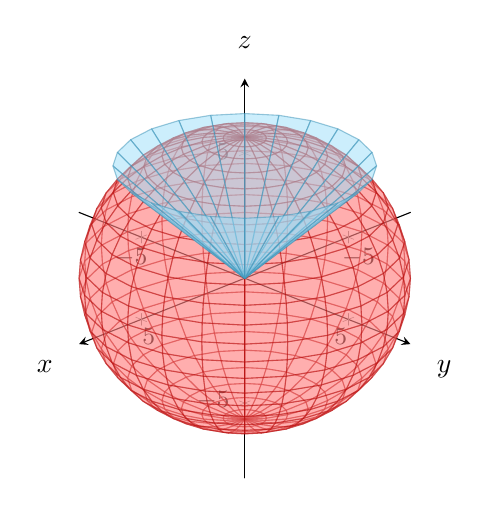
\begin{tikzpicture}[line cap=round, line join=round]
        \begin{axis}[
            view={135}{25}, % Cámara clásica
            width=10cm,
            height=10cm,
            axis lines=center,
            % 1. Ajustamos los ejes al nuevo tamaño de la esfera (aprox 5.65)
            xmin=-8, xmax=8, 
            ymin=-8, ymax=8,
            zmin=-8, zmax=8,
            xlabel={$x$},
            ylabel={$y$},
            zlabel={$z$},
            every axis x label/.style={at={(ticklabel* cs:1.05)},anchor=north east},
            every axis y label/.style={at={(ticklabel* cs:1.05)},anchor=north west},
            every axis z label/.style={at={(ticklabel* cs:1.05)},anchor=south},
            ticklabel style={font=\small},
        ]

        % Esfera de radio \sqrt{32} (Roja transparente)
        \addplot3[
            surf,
            opacity=0.4,
            color=red!50,
            faceted color=red!70!black,
            samples=25, 
            domain=0:360,
            y domain=0:180,
            z buffer=sort
        ]
        ({sqrt(32)*cos(x)*sin(y)}, {sqrt(32)*sin(x)*sin(y)}, {sqrt(32)*cos(y)});

        % Cono Superior z = \sqrt{x^2+y^2} (Celeste transparente)
        \addplot3[
            surf,
            opacity=0.5,
            color=cyan!40,
            faceted color=cyan!70!black,
            samples=25,
            samples y=2, 
            domain=0:360,
            % 2. El cono se interseca en z=4. Le damos hasta 4.5 para que lo atraviese bien
            y domain=0:4.5, 
            z buffer=sort
        ]
        ({y*cos(x)}, {y*sin(x)}, {y});

        \end{axis}
    \end{tikzpicture}
    \caption{Representación de la región pedida. \href{https://www.geogebra.org/m/pvzc3wke}{Ver en GeoGebra}}
    \label{fig:ejercicio30_figura}
\end{figure}